\chapter{Interlude: a list of examples of affine schemes}
\label{ch:spec_examples}
To cement in the previous two chapters,
we now give an enormous list of examples.
Each example gets its own section,
rather than having page-long orange boxes.

In everything that follows, $k$ is any field.

\section{Example: $\Spec k$, a single point}
This one is easy: for any field $k$,
$X = \Spec k$ has a single point,
corresponding to the only proper ideal $(0)$.
There is only way to put a topology on it.

As for the sheaf,
\[ \OO_X(X) = \OO_{X,(0)} = k. \]
So the space is remembering what field it wants to be over.
If we are complex analysists,
the set of functions on a single point is $\CC$;
if we are number theoerists,
maybe the set of functions on a single point is $\QQ$.

%%fakechapter One-dimensional
\section{$\Spec \CC[x]$, a one-dimensional line}
The scheme $X = \Spec \CC[x]$ is our beloved one-dimensional line.
It consists of two types of points:
\begin{itemize}
	\ii The closed points $(x-a)$, corresponding to each
	complex number $a \in \CC$, and
	\ii The \emph{generic} point $(0)$.
\end{itemize}
As for the Zariski topology, every open set contains $(0)$,
which captures the idea it is close to everywhere:
no matter where you stand, you can still here the buzzing of the fly!
True to the irreducibility of this space,
the open sets are huge:
the proper \emph{closed sets} consist of finitely many closed points.

Here is a picture:
for lack of better place to put it,
the point $(0)$ is floating around just above the line in red.
\begin{center}
	\begin{asy}
		size(8cm);
		pair A = (-8,0); pair B = (8,0);
		draw(A--B, Arrows);
		dot("$(x)$", (0,0), dir(-90), blue);
		dot("$(x-3)$", (3,0), dir(-90), blue);
		dot("$(x+i)$", (-4,0), dir(-90), blue);
		dot("$(0)$", (0,1), dir(90), red);
		draw( (-6,0)..(-3,0.5)..(-1,1)--(1,1)--(3,0.5)--(6,0), dotted+red );
		label("$\operatorname{Spec} \mathbb C[x]$", A, dir(-90));
	\end{asy}
\end{center}

The notion of ``value at $\kp$'' works as expected.
For example, $f = x^2+5$ is a global section of $\CC[x]$.
If we evaluate it at $\kp = x-3$,
we find $f(\kp) = f \pmod \kp = x^2+5 \pmod{x-3} = 14 \pmod{x-3}$.
As \[ \CC[x] / \kp \cong \CC \qquad \text{by $x \mapsto 3$} \]
we see we are just plugging $x=3$.

Of course, the stalk at $(x-3)$ carries more information.
In this case it is $\CC[x]_{(x-3)}$.
Which means that if we stand near the point $(x-3)$,
rational functions are all fine as long as no $x-3$
appears in the denominator.
So, $\frac{x^2+8}{(x-1)(x-5)}$ is a fine example of a germ near $x=3$.

Things get more interesting if we
consider the generic point $\eta = (0)$.

What is the stalk $\OO_{X, \eta}$?
Well, it should be $\CC[x]_{(0)} = \CC(x)$,
which is the again the set of \emph{rational} functions.
And that's what you expect.
For example, $\frac{x^2+8}{(x-1)(x-5)}$
certainly describes a rational function on ``most'' complex numbers.

What happens if we evaluate the global section
$f = x^2+5$ at $\eta$?
Well, we just get $f(\eta) = x^2+5$ ---
taking modulo $0$ doesn't do much.
Fitting, it means that if you want to be able to evaluate
a polynomial $f$ at a general complex number,
you actually just need the whole polynomial
(or rational function).
We can think of this in terms of the residue field being $\CC(x)$:
\[ \kappa( (0) ) = \Frac \left( \CC[x] / (0) \right)
	\cong \Frac \CC[x] = \CC(x). \]


\section{$\Spec \RR[x]$, a one-dimensional line
with complex conjugates glued (no fear nullstellensatz)}

Despite appearances, this actually
looks almost exactly like $\Spec \CC[x]$,
even more than you expect.
The main thing to keep in mind is that now $(x^2+1)$
is a point, which you can loosely think of as $\pm i$.
So it almost didn't matter that $\RR$ is not algebraically closed;
the $\CC$ is showing through anyways.
But this time, because we only consider
real coefficient polynomials,
we do not distinguish between ``conjugate'' $+i$ and $-i$.
Put another way, we have folded $a+bi$ and $a-bi$ into a single point:
$(x+i)$ and $(x-i)$ merge to form $x^2+1$.

To be explicit, there are three types of points:
\begin{itemize}
	\ii $(x-a)$ for each real number $a$
	\ii $(x^2-ax+b)$ if $a^2 < 4b$, and
	\ii the generic point $(0)$, again.
\end{itemize}
The ideals $(x-a)$ and $(x^2-ax+b)$
are each closed points:
the quotients with $\RR[x]$ are both fields
($\RR$ and $\CC$, respectively).


We have been drawing $\Spec \CC[x]$ as a one-dimensional line,
so $\Spec \RR[x]$ will be drawn the same way.
\begin{center}
	\begin{asy}
		size(8cm);
		pair A = (-8,0); pair B = (8,0);
		draw(A--B, Arrows);
		dot("$(x)$", (0,0), dir(-90), blue);
		dot("$(x-3)$", (3,0), dir(-90), blue);
		dot("$(x^2+1)$", (-4,0), dir(-90), blue);
		dot("$(0)$", (0,1), dir(90), red);
		draw( (-6,0)..(-3,0.5)..(-1,1)--(1,1)--(3,0.5)--(6,0), dotted+red );
		label("$\operatorname{Spec} \mathbb R[x]$", A, dir(-90));
	\end{asy}
\end{center}

One nice thing about this is that the nullstellensatz
is less scary than it was with classical varieties.
The short version is that the function $x^2+1$
vanishes at a point of $\Spec \RR[x]$,
namely $(x^2+1)$ itself!

You might remember a long time ago we made a big fuss about
the weak nullstellensatz, for example in
\Cref{pr:complex_variety_nonempty}:
if $I$ was a proper ideal in $\CC[x_1, \dots, x_n]$
there was \emph{some} point $(a_1, \dots, a_n) \in \CC^n$
such that $f(a_1, \dots, a_n) = 0$ for all $f \in I$.
With schemes, it doesn't matter anymore:
if $I$ is a proper ideal of a ring $A$,
then some maximal ideal contains it,
and so $\VV(I)$ is nonempty in $\Spec A$.

\section{$\Spec k[x]$, over any ground field}
In general, if $\ol k$ is the algebraic closure of $k$,
then $\Spec k[x]$ looks like $\Spec \ol k[x]$
with all the Galois conjugates glued together.
So we will almost never need ``algebraically closed''
hypotheses anymore: we're working with polynomial ideals,
so all the elements are implicitly there, anyways.

\section{$\Spec \ZZ$, a one-dimensional scheme}
The great thing about $\Spec \ZZ$ is that
it basically looks like $\Spec k[x]$, too,
being a one-dimensional scheme.
It has two types of prime ideals:
\begin{itemize}
	\ii $(p)$, for every rational prime $p$,
	\ii and the generic point $(0)$.
\end{itemize}
So the picture almost does not change.
\begin{center}
	\begin{asy}
		size(8cm);
		pair A = (-8,0); pair B = (8,0);
		draw(A--B, Arrows);
		dot("$(7)$", (0,0), dir(-90), blue);
		dot("$(3)$", (3,0), dir(-90), blue);
		dot("$(19)$", (-4,0), dir(-90), blue);
		dot("$(0)$", (0,1), dir(90), red);
		draw( (-6,0)..(-3,0.5)..(-1,1)--(1,1)--(3,0.5)--(6,0), dotted+red );
		label("$\operatorname{Spec} \mathbb R[x]$", A, dir(-90));
	\end{asy}
\end{center}
This time $\eta = (0)$ has stalk $\ZZ_{(0)} = \QQ$,
so a ``rational function'' is literally a rational number!
Thus, $\frac{20}{19}$ is a function
with a double root at $(2)$, a root at $(5)$,
and a simple pole at $(19)$.
If we evaluate it at $\kp = (3)$, we get $2 \pmod 3$.

The stalk $X_{(3)}$ is the rational numbers
that don't have a pole at $3$.

%%fakechapter 0D from 1D
\section{$\Spec k[x] / (x^2-x)$, two points}
If we were working with affine varieties,
you would already know what the answer is:
$x^2-x = 0$ has solutions $x=0$ and $x=1$,
so this should be a scheme with two points.

To see this come true, we use \Cref{prop:prime_quotient}:
the points of $\Spec k[x]/(x^2-x)$
should correspond to prime ideals of $k[x]$
contained in $(x^2-x)$.
As $k[x]$ is a PID, there are only two, $(x-1)$ and $(x)$.
They are each maximal,
since their quotient with $k[x]$ is a field (namely $k$),
so as promised $\Spec k[x] / (x^2-x)$ has just two closed points.

Each point has a stalk above it isomorphic to $k$.
A section on the whole space $X$ is just a choice
of two values, one at $(x)$ and one at $(x-1)$.
\begin{center}
\begin{asy}
	size(3cm);
	draw("$k$", (-2,0)--(-2,5), dir(180), red);
	draw("$k$", (2,0)--(2,5), red);
	dot("$(x)$", (-2,0), dir(-90), blue);
	dot("$(x-1)$", (2,0), dir(-90), blue);
	label("$\operatorname{Spec} k[x]/(x^2-x)$", (0,5), 2*dir(90));
\end{asy}
\end{center}
So actually, this is a geometric way of thinking about the
ring-theoretic fact that
\[ k[x] / \left( x^2-x \right) \cong k \times k
	\quad\text{by } f \mapsto \left( f(0), f(1) \right).  \]

Also, this is the first example of a reducible space in this chapter:
in fact $X$ is even disconnected.
Accordingly there is no generic point floating around:
as the space is discrete, all points are closed.

\section{$\Spec k[x]/(x^2)$, the double point}
We can now elaborate on the ``double point'' scheme
\[ X_2 = \Spec k[x] / (x^2) \]
since it is such an important motivating example.
How it does differ from the ``one-point'' scheme
$X_1 = \Spec k[x] / (x) = \Spec k$?
Both $X_2$ and $X_1$ have exactly one point,
and so obviously the topologies are the same too.

The difference is that the stalk
(equivalently, the section, since we have only one point)
is larger:
\[ \OO_{X_2, (x)} = \OO_{X_2}(X_2)  = k[x]/(x^2). \]
So to specify a function on a double point,
you need to specify two parameters, not just one:
if we take a polynomial
\[ f = a_0 + a_1 x + \dots \in k[x] \]
then evaluating it at the double point
will remember both $a_0$ and the ``first derivative'' say.

I should mention that if you drop all the way to the residue
field, you can't tell the difference between
the double point and the single point anymore.
For the residue field of $\Spec k[x] / (x^2)$ at $(x)$ is
\[ \Frac\left( A / (x) \right) = \Frac k = k. \]
Thus the set of \emph{values} is still just $k$;
but the stalk, having enriched values, can tell the difference.

\section{$\Spec k[x]/(x^3-x)$, a double point and a single point}
There is no problem putting the previous two examples side by side:
the scheme $X = \Spec k[x] / (x^3-x)$
consists of a double point next to a single point.
Note that the stalks are different:
the one above the double point is larger.
\begin{center}
\begin{asy}
	size(5cm);
	draw("$k[x] / (x^2)$", (-2,0)--(-2,7), dir(180), red);
	draw("$k$", (2,0)--(2,5), red);
	dot("$(x)$", (-2,0), dir(-90), blue+5);
	dot("$(x-1)$", (2,0), dir(-90), blue);
	label("$\operatorname{Spec} k[x]/(x^3-x)$", (0,7), 2*dir(90));
\end{asy}
\end{center}
This time, we implicitly have the ring isomorphism
\[ k[x] / (x^3-x) \cong k[x] / (x^2) \times k \]
by $f \mapsto \left( f(0) + f'(0) x, f(1) \right)$.
The derivative is meant formally here!

\section{$\Spec \Zc{60}$, a scheme with three points}
We've being seeing geometric examples of ring products coming up,
but actually the Chinese remainder theorem you are used to
with integers is no different.
(This example $X = \Spec \Zc{60}$
is taken from \cite[\S4.4.11]{ref:vakil}.)

By \Cref{prop:prime_quotient},
the prime ideals of $\Zc{60}$ are $(2)$, $(3)$, $(5)$.
But you can think of this also as coming out of $\Spec \ZZ$:
as $60$ was a function with a double root at $(2)$,
and single roots at $(3)$ and $(5)$.
\begin{center}
\begin{asy}
	size(6cm);
	draw("$\mathbb Z / 4 \mathbb Z$", (-2,0)--(-2,7), dir(180), red);
	draw("$\mathbb Z / 3 \mathbb Z$", (0,0)--(0,5), red);
	draw("$\mathbb Z / 5 \mathbb Z$", (2,0)--(2,6), red);
	dot("$(2)$", (-2,0), dir(-90), blue+5);
	dot("$(3)$", ( 0,0), dir(-90), blue);
	dot("$(5)$", ( 2,0), dir(-90), blue);
	label("$\operatorname{Spec} \mathbb Z / 60 \mathbb Z$", (0,7), 2*dir(90));
\end{asy}
\end{center}
Actually, although I have been claiming the ring isomorphisms,
the sheaves really actually give us a full proof.
Let me phrase it in terms of global sections:
\begin{align*}
	\Zc{60} &= \OO_X(X) \\
	&= \OO_X( \{(2)\} ) \times \OO_X( \{(3)\} ) \times \OO_X( \{(5)\} ) \\
	&= \OO_{X,(2)} \times \OO_{X,(3)} \times \OO_{X,(5)} \\
	&= \Zc4 \times \Zc3 \times \Zc5.
\end{align*}
So the theorem that $\OO_X(X) = A$ for $X = \Spec A$
is doing the ``work'' here;
the sheaf axioms then give us the Chinese remainder theorem from here.

%%fakechapter Two-dimensional
\section{$\Spec k[x,y]$, the two-dimensional plane}
We have seen this scheme already: it is visualized as a plane.
There are three types of points:
\begin{itemize}
	\ii The closed points $(x-a, y-b)$,
	which consists of single points of the plane.
	\ii A non-closed point $(f(x,y))$ for any irreducible
	polynomial $f$, which floats along some irreducible curve.
	We illustrate this by drawing the dotted curve along
	which the point is floating.
	\ii The generic point $(0)$, floating along the entire plane.
	I don't know a good place to put it in the picture,
	so I'll just put it somewhere and draw a dotted circle around it.
\end{itemize}

Here is an illustration of all three types of points.
\begin{center}
\begin{asy}
	graph.xaxis();
	graph.yaxis();
	real f(real x) { return x*x; }
	graph.xaxis("$x$");
	graph.yaxis("$y$");
	draw(graph(f,-2,2,operator ..), blue+dotted, Arrows(TeXHead));
	dot("$(y-x^2)$", (1.3, f(1.3)), dir(-45), blue);
	dot("$(x-1,y+2)$", (1,-2), dir(-45), red);
	pair O = (-3,3);
	dot("$(0)$", O, dir(225), deepgreen);
	filldraw(CR(O, 0.8), opacity(0.2)+lightgreen, dotted+green);
\end{asy}
\end{center}

We also go ahead and compute the stalks above each point.
\begin{itemize}
	\ii The stalk above $(x-1, y+2)$ is
	the set of rational functions $\frac{f(x,y)}{g(x,y)}$
	such that $g(1,-2) \ne 0$.
	\ii The stalk above the non-closed point $(y-x^2)$
	the set of rational functions $\frac{f(x,y)}{g(x,y)}$
	such that $g(t, t^2) \ne 0$.
	For example the function $\frac{xy}{x+y-2}$ is still fine;
	despite the fact it vanishes at the point $(1,1)$ and $(-2,4)$
	on the parabola it is a function
	on a ``generic point'' (crudely, ``most points'') of the parabola.
	\ii The stalk above $(0)$ is the entire fraction field
	$k(x,y)$ of rational functions.
\end{itemize}

Let's consider the global section $f = x^2 + y^2$
and also take the value at each of the above points.
\begin{itemize}
	\ii $f \pmod{x-1,y-2} = 5$, so $f$ has value $5$ at $(x-1, y+2)$.
	\ii The new bit is that we can think of evaluating
	$f$ along the parabola too --- it is given a particular value
	in the quotient $k[x,y] / (y-x^2)$.
	We can think of it as $f = x^2+y^2 \equiv x^2+x^4 \pmod{y-x^2}$ for example.
	Note that if we know the value of $f$ at the generic point of the parabola,
	we can therefore also evaluate it at any closed point on the parabola.
	\ii At the generic point $(0)$, $f \pmod{0} = f$.
	So ``evaluating at the generic point'' does nothing, as in any other scheme.
\end{itemize}


\section{$\Spec \ZZ[x]$, a two-dimensional scheme, and Mumford's picture}
We saw $\Spec \ZZ$ looked a lot like $\Spec k[x]$,
and we will now see that $\Spec \ZZ[x]$ looks a lot like $\Spec k[x,y]$.
As before, there are there types of prime ideals,
but they will look somewhat more different:
\begin{itemize}
	\ii The closed points are now pairs $(p, f(x))$
	where $p$ is a prime and $f$ is an irreducible polynomial modulo $p$.
	Indeed, these are the maximal ideals:
	the quotient $\ZZ[x] / (p,f)$ becomes some finite extension of $\FF_p$.
	\ii There are now two different ``one-dimensional'' non-closed points:
	\begin{itemize}
		\ii Each rational prime gives a point $(p)$ and
		\ii Each irreducible polynomial $f$ gives a point $(f)$.
	\end{itemize}
	Indeed, note that the quotients of $\ZZ[x]$ by each are integral domains.
	\ii $\ZZ[x]$ is an integral domain,
	so as always $(0)$ is our generic point for the entire space.
\end{itemize}

There is a famous picture of this scheme in Mumford's ``red book'',
which I will produce here for culture-preservation reasons,
even though there are some discrepancies between
the pictures that we previously drew.
\begin{center}
	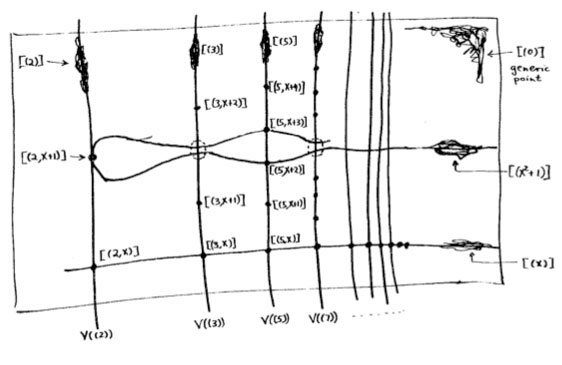
\includegraphics[width=0.9\textwidth]{media/mumforddrawing.jpg}
\end{center}
Mumford uses $[\kp]$ to denote the point $\kp$,
which we don't, so you can ignore the square brackets that appear everywhere.
The non-closed points are illustrated as balls of fuzz.
There is one bit that I would do differently,
in $V(3)$ and $V(7)$, there ought to be a point $(3,x^2+1)$,
which is not drawn as a closed point in the picture,
but rather as dashed oval.
This is not right in the topological sense:
as $\km = (3, x^2+1)$ is a maximal ideal,
so it really is one closed point in the scheme.
But the reason it might be thought of as counting as two points
is that $\ZZ[x] / (3,x^2+1)$,
the field of possible values at $\km$,
is a two-dimensional $\FF_3$ vector space.



%%fakechapter 1D cut out from 2D
\section{$\Spec k[x,y]/(y-x^2)$, the parabola}
\section{$\Spec k[x,y]/(xy)$, two axes}
\section{$\Spec \ZZ[i]$, the Gaussian integers (one-dimensional)}
\section{$\Spec k[x] \times k[y]$, two ``parallel'' lines}

%%fakechapter 1D with holes
\section{$\Spec k[x]_x$, the punctured line (or hyperbola)}
\section{$\Spec \ZZ_{55}$, deleting $5$ and $11$}
\section{$\Spec (k[x,y]/(xy))_{x+y}$, two axes with the origin deleted}

%%fakechapter 0D --- stalks above 1D
\section{$\Spec k[x]_{(x)}$, the stalk above the origin}
\section{$\Spec k[x]_{(0)}$, the stalk above the generic point}
\section{$\Spec \ZZ_{(5)}$, the stalk above $(5)$}
\section{$\Spec \ZZ_{(0)} = \Spec \QQ$}
\section{$\Spec k[x,y]_{(x,y)}$, the stalk above the origin}
\section{$\Spec k[x,y]_{(y-x^2)}$, the stalk above the parabola}
\section{$\Spec k[x,y]_{(0)}$, the stalk above the generic point}

